%
\documentclass{report}
\usepackage{setspace}
%\usepackage{subfigure}

\pagestyle{plain}
\usepackage{amssymb,graphicx,color}
\usepackage{amsfonts}
\usepackage{latexsym}
\usepackage{a4wide}
\usepackage{amsmath}

\graphicspath{{figures/}}

\usepackage{hyperref}
\usepackage[all]{hypcap}

\usepackage[utf8]{inputenc}
\usepackage[english]{babel}
\usepackage[nottoc]{tocbibind}

\newtheorem{theorem}{THEOREM}
\newtheorem{lemma}[theorem]{LEMMA}
\newtheorem{corollary}[theorem]{COROLLARY}
\newtheorem{proposition}[theorem]{PROPOSITION}
\newtheorem{remark}[theorem]{REMARK}
\newtheorem{definition}[theorem]{DEFINITION}
\newtheorem{fact}[theorem]{FACT}

\newtheorem{problem}[theorem]{PROBLEM}
\newtheorem{exercise}[theorem]{EXERCISE}
\def \set#1{\{#1\} }

\newenvironment{proof}{
PROOF:
\begin{quotation}}{
$\Box$ \end{quotation}}



\newcommand{\nats}{\mbox{\( \mathbb N \)}}
\newcommand{\rat}{\mbox{\(\mathbb Q\)}}
\newcommand{\rats}{\mbox{\(\mathbb Q\)}}
\newcommand{\reals}{\mbox{\(\mathbb R\)}}
\newcommand{\ints}{\mbox{\(\mathbb Z\)}}

%%%%%%%%%%%%%%%%%%%%%%%%%%


\title{         { 
\includegraphics[scale=.5]{ucl_logo.png}}\\
{{\Huge Multi-hop Question Answering on Graph Completed with Reinforcement Learning}}\\
% {\large Optional Subtitle}\\
                }
\date{September 2019}
\author{Yangguang Li\thanks{
{\bf Disclaimer:}
This report is submitted as part requirement for the MSc in Computational Statistics and Machine Learning at UCL. It is
substantially the result of my own work except where explicitly indicated in the text. The report may be freely copied and distributed provided the source is explicitly acknowledged}
\\ \\
MSc Computational Statistics and Machine Learning\\ \\
Supervisor: Prof. Philip Treleaven\\
Industrial Supervisor: Marcelo Gutierrez}



\begin{document}

 \onehalfspacing
\maketitle
\begin{abstract}
\begin{singlespace}
This dissertation investigates the possibility of utilizing link prediction on graphs as an auxiliary task of multi-hop question answering (MHQA) problem, i.e. to improve MHQA by completing the graph used for inference. Another sub-goal is to examine ways to adapt reinforcement learning for predicting links on knowledge graphs (KG). This is important as multi-hop question answering, or reading comprehension, has imposed a bigger challenge over single-document question answering problems. In the single document setting, well-developed models are able to achieve human-level performance, but fall behind in the multi-document setting. Although some researches have started to tackle this problem, they are far from achieving human-level performance, not mention to solve it. Also link prediction, especially on KGs, is useful for recommendation systems, search engine, just to name a few. KGs are known to be incomplete, the ability to reason what is missing in them automatically is vital for successful application of KG in those fields mentioned.

One of the challenge in the MHQA problem is the ability to reason across multiple documents. Some researchers have tried to tackle this problem by using multi-hop attention networks to gather information from documents step-by-step before getting the conclusion. Another way proposed to solve this problem is to frame it as an inference problem on graphs. Following the resurgent of graph neural network (GNN), researchers experimented with running GNN algorithms on the graph extracted from the supporting documents.

This research comprises constructing the graphs from supporting documents, performing link prediction on the constructed graphs, and doing inference on the completed graphs using GNNs. The graphs used are heterogenous and they encode the information extracted from the supporting documents, where the nodes are entities, candidate answers for the question (as \textbf{candidates} below), and documents. The edges are seven kinds of relationships between the nodes including: i. document-candidate edge if the candidate appears in the document for at least once; ii. document-entity edge if the entity appears in the document; iii. candidate-entity edge if the candidate is a exact match of the extracted entity; iv. entity-entity edge if they appear in the same document; v. cross-document coreference edge if the two entities are on the same coreference
chain but are in different documents; vi. candidate-candidate edge where all candidates are connected; vii. complement edge which connected all nodes that are not adjacent to any other kind of edges.

[\textbf{TODO} link prediction]

Once the graph is completed, GNNs are run on the graph to do inference, i.e. try to answer the question by picking one of the candidates. Particularly, graph convolutional networks (GCN), graph recurrent networks (GRN), and graph attention networks (GAT) have been experimented to solve the inference problem. The whole system is tested and evaluated on QAngaroo and HOTPOTQA which are specifically constructed datasets for MHQA.

\end{singlespace}
\end{abstract}
\tableofcontents
% \setcounter{page}{1}
\listoffigures
% \listoftables


\chapter{Introduction}
Being able to build a system that can read in textual corpus, reason on it, and achieve a conclusion is a longstanding goal in the fields of information retrieval and natural language processing (NLP). A way to assess such a system is by evaluating its performance on question answering (QA) datasets. Such a dataset is specifically prepared as a set of questions $\{A\}$, where each question $A$ consists of a query $q$ and the correct answer $\bar{c}$. Sometimes there may also be supporting document(s) $\{d\}$ and a list of candidates $\{c\}$ being provided. The system is required to answer the query based on the supporting document(s) or some common knowledge/knowledge bases it has in itself. If the candidates is provided the system just need to pick one of them; otherwise it needs to extract the correct answer of free-form text from the whole span of the given text.

Previous researches mainly focused on QA based on only a single document or paragraph. Boosted by the availability of large-scale datasets like SQuAD \cite{rajpurkar_squad:_2016} and CNN/Daily Mail \cite{hermann_teaching_2015} which contain questions that can be answered by attending the information in only one single sentence,  many end-to-end neural models \cite{seo_bidirectional_2016, xiong_dynamic_2016, shen_reasonet:_2017} have been proposed and achieved good performances on these datasets. To overcome the limit of these datasets \cite{weissenborn_making_2017}: requiring only the information from one single sentence to answer the questions, people have proposed NarrativeQA \cite{kocisky_narrativeqa_2018}, CoQA \cite{reddy_coqa:_2019}, TriviaQA \cite{joshi_triviaqa:_2017}, and RACE \cite{lai_race:_2017} which have questions that can only be answered if information from multiple sentences within the same document is gathered together.

Although remaining challenging, these datasets are created for reasoning within the same document, which is not the case for many real-world applications that requires aggregating information from multiple documents, or even from multimodal sources. In this dissertation we only focus on text question answering, hence only tackling the case of multi-document QA. Seeing the need for a dataset to facilitate research in MHQA, Welbl et al. released a new dataset named QAngaroo \cite{welbl_constructing_2018} which consists of WikiHop and MedHop. The dataset requires the system to reason across multiple supporting documents before it can achieve the conclusion to pick the right answer among the candidates. WikiHop consists of questions generated from the user-created multi-domain unstructured text corpus Wikipedia and the structured information set Wikidata. All the information needed for answering a particular query is contained in the supporting documents, but there may also be some misleading documents which penalise the systems that perform only exact matches without comprehending the context in the reasoning procedure. In Figure \ref{wikihop_example}, we show an example of WikiHop dataset where the system need to combine information from several documents to get the correct answer to the question. We can also see the appearance of misleading document in the example: in the first document we get \textit{Mumbai} is adjacent to the \textit{Arabian Sea}, and in the last document we find that \textit{Arabian Sea} is closer to \textit{Pakistan} and \textit{Iran} than the correct answer, \textit{India}, does in terms of the relational positions in the text. In such a scenario, a system that does not have semantic understanding of the context may fall into the trap and pick \textit{Iran} or \textit{Pakistan} as the answer. The MedHop dataset in QAngaroo is about finding the drug that will interact with a given drug according the provided text from PubMed, a dataset of biomedical literatures. The supporting documents are abstracts of research papers, and al candidates are drugs' names extracted from the whole text corpus. This dataset is much smaller comparing to WikiHop: 2,508 instances versus the 51,318 ones of the WikiHop. Also the text are closed-domain now, hence the requirement on the ability to do reading comprehension is lower than that of WikiHop. 
\begin{figure}
\centering
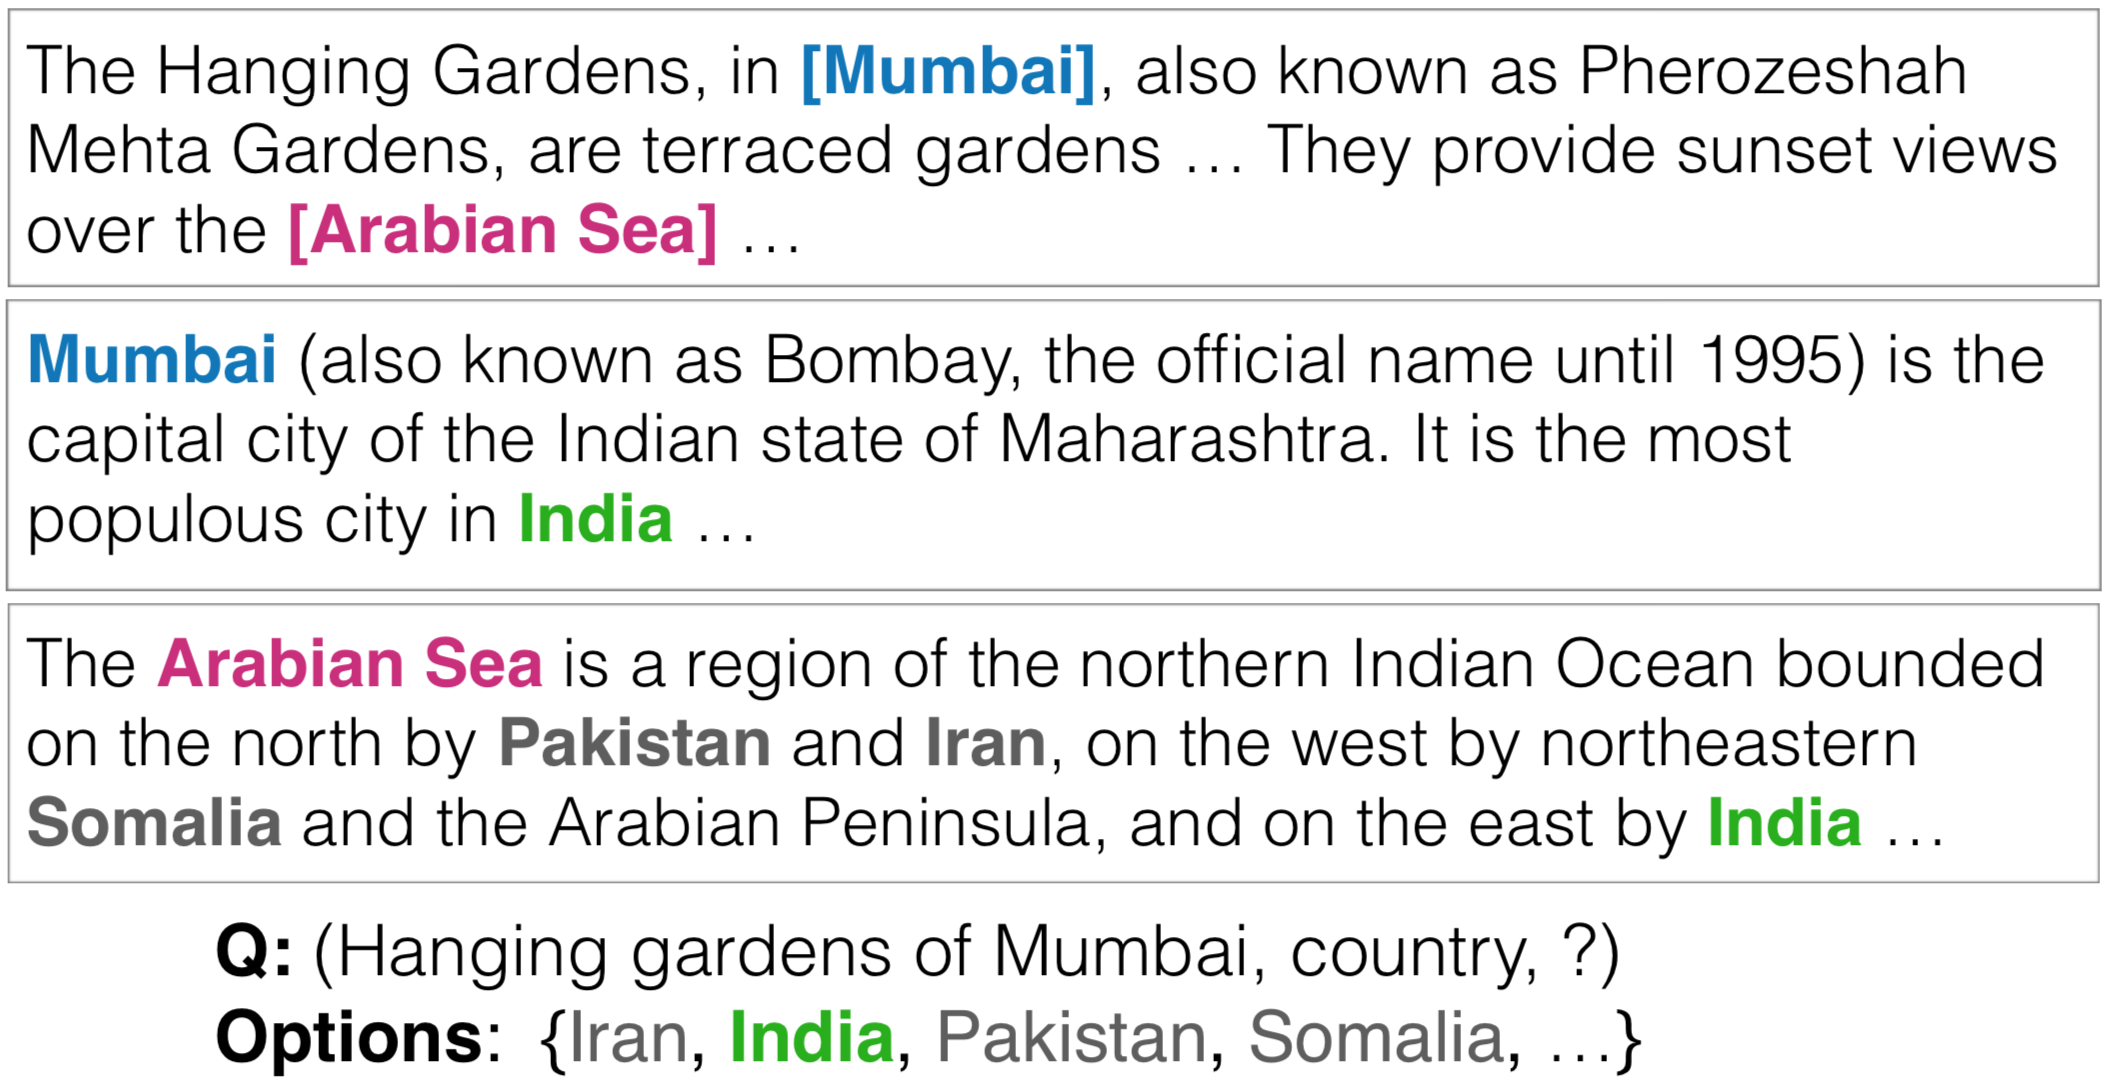
\includegraphics[width=0.9\textwidth]{figures/wikihop_example.png}
\label{wikihop_example}
\caption[An example from the WikiHop dataset.]{An example from the WikiHop dataset. Reprinted from \cite{welbl_constructing_2018}.}
\end{figure}

[\textbf{TODO}: HotpotQA]




\chapter{Related Work}

\chapter{Methodology}
This chapter consists of detailed descriptions of the model design, implementation, testing, and a discussion of the contribution of this dissertation.

\section{Model Design}

\chapter{Experimental Results}

\chapter{Conclusion}

\appendix
\bibliographystyle{plain}
\bibliography{ref}

%\chapter{Appendix}

\end{document}
